\documentclass{article}\usepackage[]{graphicx}\usepackage[]{color}
%% maxwidth is the original width if it is less than linewidth
%% otherwise use linewidth (to make sure the graphics do not exceed the margin)
\makeatletter
\def\maxwidth{ %
  \ifdim\Gin@nat@width>\linewidth
    \linewidth
  \else
    \Gin@nat@width
  \fi
}
\makeatother

\definecolor{fgcolor}{rgb}{0.345, 0.345, 0.345}
\newcommand{\hlnum}[1]{\textcolor[rgb]{0.686,0.059,0.569}{#1}}%
\newcommand{\hlstr}[1]{\textcolor[rgb]{0.192,0.494,0.8}{#1}}%
\newcommand{\hlcom}[1]{\textcolor[rgb]{0.678,0.584,0.686}{\textit{#1}}}%
\newcommand{\hlopt}[1]{\textcolor[rgb]{0,0,0}{#1}}%
\newcommand{\hlstd}[1]{\textcolor[rgb]{0.345,0.345,0.345}{#1}}%
\newcommand{\hlkwa}[1]{\textcolor[rgb]{0.161,0.373,0.58}{\textbf{#1}}}%
\newcommand{\hlkwb}[1]{\textcolor[rgb]{0.69,0.353,0.396}{#1}}%
\newcommand{\hlkwc}[1]{\textcolor[rgb]{0.333,0.667,0.333}{#1}}%
\newcommand{\hlkwd}[1]{\textcolor[rgb]{0.737,0.353,0.396}{\textbf{#1}}}%
\let\hlipl\hlkwb

\usepackage{framed}
\makeatletter
\newenvironment{kframe}{%
 \def\at@end@of@kframe{}%
 \ifinner\ifhmode%
  \def\at@end@of@kframe{\end{minipage}}%
  \begin{minipage}{\columnwidth}%
 \fi\fi%
 \def\FrameCommand##1{\hskip\@totalleftmargin \hskip-\fboxsep
 \colorbox{shadecolor}{##1}\hskip-\fboxsep
     % There is no \\@totalrightmargin, so:
     \hskip-\linewidth \hskip-\@totalleftmargin \hskip\columnwidth}%
 \MakeFramed {\advance\hsize-\width
   \@totalleftmargin\z@ \linewidth\hsize
   \@setminipage}}%
 {\par\unskip\endMakeFramed%
 \at@end@of@kframe}
\makeatother

\definecolor{shadecolor}{rgb}{.97, .97, .97}
\definecolor{messagecolor}{rgb}{0, 0, 0}
\definecolor{warningcolor}{rgb}{1, 0, 1}
\definecolor{errorcolor}{rgb}{1, 0, 0}
\newenvironment{knitrout}{}{} % an empty environment to be redefined in TeX

\usepackage{alltt}
\usepackage{amscd, amssymb, amsmath, verbatim, setspace}
\usepackage[left=1.0in, right=1.0in, top=1.0in, bottom=1.0in]{geometry}
\usepackage{mathrsfs}
\usepackage{listings}


\IfFileExists{upquote.sty}{\usepackage{upquote}}{}
\begin{document}
\begin{flushright}
Arif Ali\\
Math 611 Stochastic Simulation\\
Oct 27, 2016\\
\end{flushright}

\begin{center}
\LARGE\textbf{Homework 7}
  \end{center}
\section*{Exercise 1 \& 2}
\subsection*{Part A}
\begin{knitrout}
\definecolor{shadecolor}{rgb}{0.969, 0.969, 0.969}\color{fgcolor}\begin{kframe}
\begin{alltt}
\hlstd{f} \hlkwb{=} \hlkwa{function}\hlstd{(}\hlkwc{x}\hlstd{)} \hlkwd{dgamma}\hlstd{(x,} \hlnum{4.3}\hlstd{,}\hlnum{6.2}\hlstd{)}
\hlstd{g} \hlkwb{=} \hlkwa{function}\hlstd{(}\hlkwc{x}\hlstd{)} \hlkwd{dgamma}\hlstd{(x,} \hlnum{4}\hlstd{,} \hlnum{7}\hlstd{)}


\hlstd{Nsim}\hlkwb{=}\hlnum{10}\hlopt{^}\hlnum{4}
\hlstd{X}\hlkwb{=}\hlkwd{rgamma}\hlstd{(}\hlnum{1}\hlstd{,} \hlnum{4.3}\hlstd{,}\hlnum{6.2}\hlstd{)}    \hlcom{# initialize the chain from the stationary}
\hlstd{accept} \hlkwb{=} \hlkwd{c}\hlstd{(}\hlnum{0}\hlstd{)}
\hlkwa{for} \hlstd{(t} \hlkwa{in} \hlnum{2}\hlopt{:}\hlstd{Nsim)\{}
  \hlstd{Y}\hlkwb{=}\hlkwd{rgamma}\hlstd{(}\hlnum{1}\hlstd{,} \hlnum{4}\hlstd{,}\hlnum{7}\hlstd{)}   \hlcom{# candidate normal}
  \hlstd{rho}\hlkwb{=}\hlkwd{f}\hlstd{(Y)}\hlopt{*}\hlkwd{g}\hlstd{(X[t}\hlopt{-}\hlnum{1}\hlstd{])}\hlopt{/}\hlstd{(}\hlkwd{f}\hlstd{(X[t}\hlopt{-}\hlnum{1}\hlstd{])}\hlopt{*}\hlkwd{g}\hlstd{(Y))}
  \hlkwa{if}\hlstd{(}\hlkwd{runif}\hlstd{(}\hlnum{1}\hlstd{)}\hlopt{<}\hlstd{rho)\{}
    \hlstd{X[t]} \hlkwb{=} \hlstd{Y}
    \hlstd{accept[t]} \hlkwb{=} \hlnum{1}
  \hlstd{\}}
  \hlkwa{else}\hlstd{\{}
    \hlstd{X[t]} \hlkwb{=}\hlstd{X[t}\hlopt{-}\hlnum{1}\hlstd{]}
    \hlstd{accept[t]} \hlkwb{=} \hlnum{0}
  \hlstd{\}}
\hlstd{\}}
\hlkwd{plot}\hlstd{(X,} \hlkwc{type} \hlstd{=} \hlstr{"l"}\hlstd{,}
     \hlkwc{main} \hlstd{=} \hlstr{"target distribution gamma(4.3,6.2) with candidate gamma(4, 7)"}\hlstd{,}
     \hlkwc{xlab} \hlstd{=} \hlstr{"iteration"}\hlstd{)}
\hlkwd{abline}\hlstd{(}\hlkwc{h} \hlstd{=} \hlnum{4.3}\hlopt{/}\hlnum{6.2}\hlstd{,} \hlkwc{col} \hlstd{=} \hlstr{"red"}\hlstd{)}
\end{alltt}
\end{kframe}
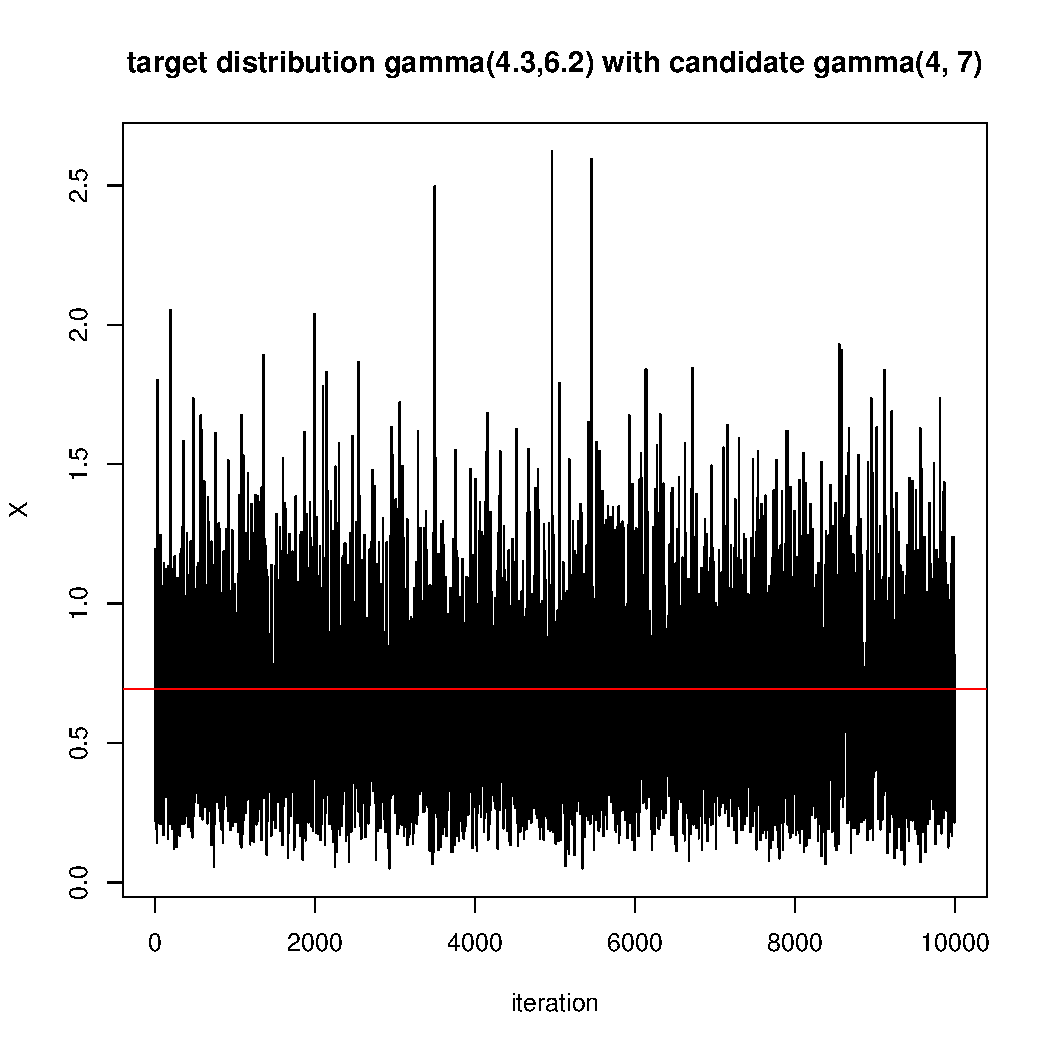
\includegraphics[width=0.60\linewidth]{figure/unnamed-chunk-2-1} 

\end{knitrout}
From the Metropolis-Hastings Algorithm the estimated mean of $gamma(4.3,6.2)$ is 0.6950373 and the acceptance rate is 77.97\%.
\subsection*{Part B}
\begin{knitrout}
\definecolor{shadecolor}{rgb}{0.969, 0.969, 0.969}\color{fgcolor}\begin{kframe}
\begin{alltt}
\hlstd{g} \hlkwb{=} \hlkwa{function}\hlstd{(}\hlkwc{x}\hlstd{)} \hlkwd{dgamma}\hlstd{(x,}\hlnum{5}\hlstd{,}\hlnum{6}\hlstd{)}

\hlstd{X}\hlkwb{=}\hlkwd{rgamma}\hlstd{(}\hlnum{1}\hlstd{,} \hlnum{4.3}\hlstd{,}\hlnum{6.2}\hlstd{)}
\hlstd{accept} \hlkwb{=} \hlkwd{c}\hlstd{(}\hlnum{0}\hlstd{)}
\hlkwa{for} \hlstd{(t} \hlkwa{in} \hlnum{2}\hlopt{:}\hlstd{Nsim)\{}
  \hlstd{Y}\hlkwb{=}\hlkwd{rgamma}\hlstd{(}\hlnum{1}\hlstd{,} \hlnum{5}\hlstd{,}\hlnum{6}\hlstd{)}
  \hlstd{rho}\hlkwb{=}\hlkwd{f}\hlstd{(Y)}\hlopt{*}\hlkwd{g}\hlstd{(X[t}\hlopt{-}\hlnum{1}\hlstd{])}\hlopt{/}\hlstd{(}\hlkwd{f}\hlstd{(X[t}\hlopt{-}\hlnum{1}\hlstd{])}\hlopt{*}\hlkwd{g}\hlstd{(Y))}
  \hlkwa{if}\hlstd{(}\hlkwd{runif}\hlstd{(}\hlnum{1}\hlstd{)}\hlopt{<}\hlstd{rho)\{}
    \hlstd{X[t]} \hlkwb{=} \hlstd{Y}
    \hlstd{accept[t]} \hlkwb{=} \hlnum{1}
  \hlstd{\}}
  \hlkwa{else}\hlstd{\{}
    \hlstd{X[t]} \hlkwb{=}\hlstd{X[t}\hlopt{-}\hlnum{1}\hlstd{]}
    \hlstd{accept[t]} \hlkwb{=} \hlnum{0}
  \hlstd{\}}
\hlstd{\}}
\hlkwd{plot}\hlstd{(X,} \hlkwc{type} \hlstd{=} \hlstr{"l"}\hlstd{,}
     \hlkwc{main} \hlstd{=} \hlstr{"target distribution gamma(4.3,6.2) with candidate gamma(5, 6)"}\hlstd{,}
     \hlkwc{xlab} \hlstd{=} \hlstr{"iteration"}\hlstd{)}
\hlkwd{abline}\hlstd{(}\hlkwc{h} \hlstd{=} \hlnum{4.3}\hlopt{/}\hlnum{6.2}\hlstd{,} \hlkwc{col} \hlstd{=} \hlstr{"red"}\hlstd{)}
\end{alltt}
\end{kframe}
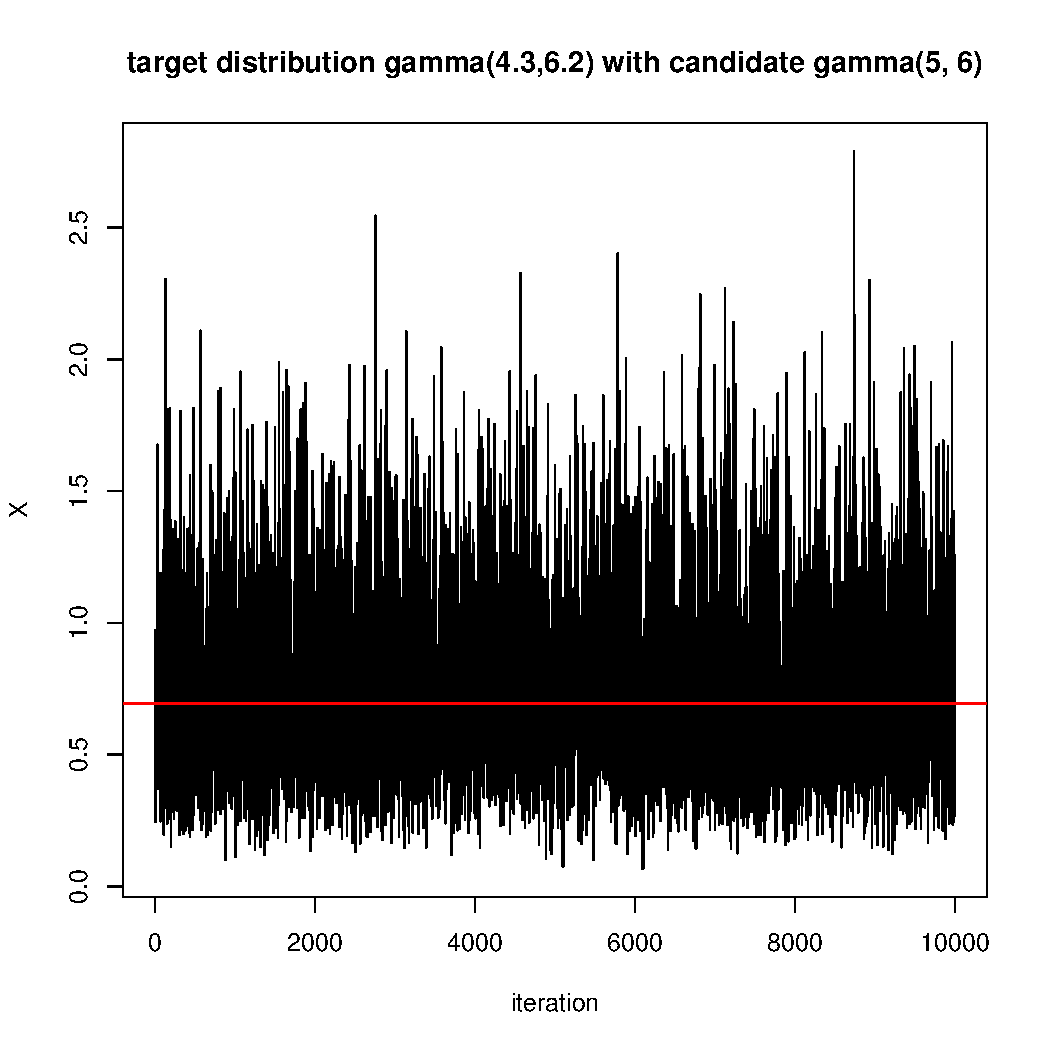
\includegraphics[width=0.60\linewidth]{figure/unnamed-chunk-3-1} 

\end{knitrout}
From the Metropolis-Hastings Algorithm the estimated mean of $gamma(4.3,6.2)$ is 0.6846806 and the acceptance rate is 75.95\%.

\section*{Exercise 3}
\begin{knitrout}
\definecolor{shadecolor}{rgb}{0.969, 0.969, 0.969}\color{fgcolor}\begin{kframe}
\begin{alltt}
\hlkwd{library}\hlstd{(}\hlstr{'mixtools'}\hlstd{)}
\end{alltt}


{\ttfamily\noindent\itshape\color{messagecolor}{\#\# mixtools package, version 1.0.4, Released 2016-01-11\\\#\# This package is based upon work supported by the National Science Foundation under Grant No. SES-0518772.}}\begin{alltt}
\hlstd{x} \hlkwb{=} \hlkwd{c}\hlstd{(}\hlnum{0.12}\hlstd{,}\hlnum{0.17}\hlstd{,}\hlnum{0.32}\hlstd{,}\hlnum{0.56}\hlstd{,}\hlnum{0.98}\hlstd{,}\hlnum{1.03}\hlstd{,}\hlnum{1.10}\hlstd{,}\hlnum{1.18}\hlstd{,} \hlnum{1.23}\hlstd{,} \hlnum{1.67}\hlstd{,} \hlnum{1.68}\hlstd{,} \hlnum{2.33}\hlstd{)}
\hlstd{out} \hlkwb{<-} \hlkwd{gammamixEM}\hlstd{(x)}
\end{alltt}
\begin{verbatim}
## number of iterations= 39
\end{verbatim}
\begin{alltt}
\hlstd{out[}\hlnum{2}\hlopt{:}\hlnum{4}\hlstd{]}
\end{alltt}
\begin{verbatim}
## $lambda
## [1] 0.2464711 0.7535289
## 
## $gamma.pars
##           comp.1    comp.2
## alpha 5.70365196 6.9064472
## beta  0.03578078 0.1884112
## 
## $loglik
## [1] -9.071738
\end{verbatim}
\end{kframe}
\end{knitrout}

$Gamma(1, \beta) \equiv Exp(\beta)$ therefore the estimates for $\mu$ and $\lambda$ are 0.0357808, 0.1884112 respectively. The one issue is that the gamma mixture gives outputs for the $\alpha$ in a gamma distribution. This is set at $\alpha = 1$ for an exponential distribution.
\section*{Exercise 4}
\subsection*{Part A}
\begin{equation}
\left[\begin{array}{ccccc}
 & 1 & 2 & 3 & 4\\
1 & 1 & 0 & 0 & 0\\
2 & 0 & 1 & 0 & 0\\
3 & 0 & 0.019 & 0.98 & 0.001\\
4 & 0.02 & 0.03 & 0 & 0.95
\end{array}\right]
\end{equation}
\begin{equation}
(I-R) = \left[\begin{array}{cc}
1-0.98 & 0-0.001\\
0-0 & 1-0.95
\end{array}\right]=\left[\begin{array}{cc}
0.02 & -0.001\\
0 & 0.05
\end{array}\right]
\end{equation}

\begin{equation}
(I-R)^{-1} = \frac{1}{0.02*0.05-(-0.001)(0)}\left[\begin{array}{cc}
0.05 & 0.001\\
0 & 0.02\end{array}\right]=\left[\begin{array}{cc}
50 & 1\\
0 & 20\end{array}\right]
\end{equation}

\begin{equation}
\left[\begin{array}{cc}
50 & 1\\
0 & 20\end{array}\right] * \left[\begin{array}{cc}
0 & 0.019\\
0.02 & 0.03\end{array}\right] = \left[\begin{array}{cc}
0.02 & 0.98\\
0.4 & 0.6\end{array}\right]
\end{equation}
\begin{equation}
P(3,1) = 0.02
\end{equation}
\subsection*{Part B}
\begin{equation}
E(3,3)=50
\end{equation}
\end{document}
